\raggedbottom
\chapter{Game Design and Mechanics}
\label{cha:games_to_be_developed}

% This chapter aims to explore in detail the mini-games to be developed. We will dive into each aspect of the mini-games, the way they're meant to be played and explaining which competeces each one aims to achieve. At the end of each explanation some screenshots of the games are displayed.

In this chapter, we take a detailed look at the mini-games developed. There will be an explanation of how each game is played and the specific skills each one aims to improve.

After describing each one, we'll display some screenshots. This way, we'll showcase a clear understanding of how the games work and the objectives they’re designed to achieve.

% TODO: PRF Terminar aqui com com um paragrafo a indicar a organizacao do capitulo, indicando o conteudo de cada seccao

% (No início do capítulo, colocar um resumo sobre o mesmo, indicando 
% o conteúdo de cada secção)
% 3.1 - Game 1 - Hearts
% 3.2 - Game 2 - Maze
% 3.3 - Game 3 - Sounds
% ...
% (Descrição de todos os jogos a desenvolver, um por cada secção específica)
% (Tentar ser coerente e consistente na descrição de todos os jogos)
% (Descrever quais as competências que o jogo visa desenvolver)
% (Descrever quais as ações que o utilizador/criança deve fazer perante o jogo
% e indicar qual o resultado - score/pontuação - do jogo)
% (Indicar as situações de sucesso/insucesso do jogo)
% (Para cada jogo, indicar também a faixa etária a que se destina)

\newpage
\section{Games Overview}
% TODO: detalhar a estrutura dos jogos

\newpage
\section{Game 1 - Hearts}

The Hearts Game is the first one and also most simplest. This is because it targeted for children between the age of 6 to 10 years old.

% Game Description
\paragraph{Description}
The game consists of multiple hearts showing up on screen, which the child must click in order to score points. When some heart isn't pressed within some time limit, it gets destroyed and decreases the score points.

The game progresses along three different levels. These levels introduce the increase of the speed the hearts spawn and also new distracting hearts that also get spawned but shouldn't be clicked, damaging the score.

Success would be when the user is able to hit most of the hearts, while failure occurs when the child hits too many distractor hearts or isn't able to hit most of the hearts present on the screen.

With this in mind, the player will have to adopt the following user actions:

\begin{itemize}
    \item \textbf{Identify and Click} the hearts on the screen.
    \item \textbf{Avoid any distractors} that may appear.
    \item \textbf{Adapt to the speed} of spawning of hearts.
\end{itemize}

\subsection*{Competences}
Despite being simple, the game allows for multiple competence acquisition from the children such as:

\paragraph{The Visual Attention and Processing Speed}- Children must identify and hit the hearts really quickly, enhancing their ability to focus and respond promptly. This is a crucial skill for children with \textbf{Visual Motor Deficit} and \textbf{Non-Verbal Learning Disabilities}.

\paragraph{Hand-Eye Coordination and Fine Motor Skills}- Each click in a heart requires precise hand-eye coordination, which helps to improve fine motor skills, greatly beneficial for children with \textbf{Dysgraphia} and \textbf{Visual Motor Deficit}.

\paragraph{Impulsivity Control and Decision Making}- As the difficulty increases, there are some hearts which should not be clicked. This challenges the child to control impulsive actions and take careful decisions. This is really beneficial for children with \textbf{ADHD} or \textbf{Non-Verbal Learning Disabilities}.

% TODO: PRF Falta falar de ADHD

% As for HUD there is a progress bar in the upper center part of the screen that increases with time and, when reaches the end means the round is over. There is also a score in the right upper side that displays the user's current score.

The following image (fig. \ref{fig:heartsGameplay}) displays a screen of the game during one of the gameplays.

\begin{figure}[H]
    \centering
    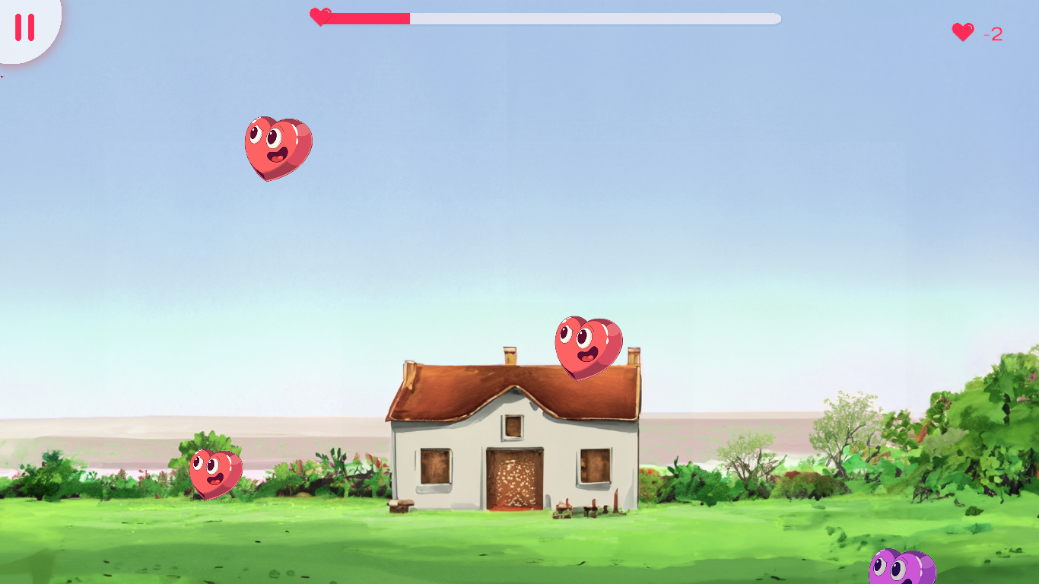
\includegraphics[scale=0.45]{Chapters/gameplay/HeartsGame.png}
    \caption{Hearts Game - Gameplay}
    \label{fig:heartsGameplay}    
\end{figure}

% TODO: PRF Adicionar mais fotos

\newpage
\section{Game 2 - Maze}

The Maze Game is designed for children between the age of 6 to 12 years old.

\paragraph{Description}

This game consists of a maze where the main character, Mr. Pig, has to navigate through a forest in order to find the exit. One of Mr. Pig's challenges is to pick up all gargabe he finds along the way, to keep nature clean.

During the game play the user's primary action is to navigate Mr. Pig through the maze using, either the arrow keys or drag and drop gestures. Before completing the maze it's expected that the player finds all the objects that are not healthy for nature.
At the end of the maze the player is met with a recycling bin for all the garbage collected.

By collecting each object in the forest, the user is met with positive reinforcement like sounds and notifications encouraging to move forward and progress to other levels. If the player fails to collect all objects in the forest before reaching the end, some feedback will show on screen to encourage the completion of the level.

This game's metric for success is the elapsed time and allows the players to complete each level at any pace, but with a highscore system keeps them motivated to beat the highest score and be faster.

\subsection*{Competences}
The following are some of the competences this game aims to improve.

\paragraph{Problem Solving}- Children must plan their route through the maze, getting to the most efficient path to collect all objects and reach the exit, which helps improve critical thinking and decision making. This can help a lot children with \textbf{Dyslexia} and \textbf{Dyscalculia}.

\paragraph{Visual-Motor Integration}- It helps to improve the coordination between visual perception and motor control. Navigating the player through the maze requires the processing of visual information about the maze's layout and respond with precise movements. This is really beneficial for children with \textbf{Visual Motor Deficit}.

\paragraph{Language Processing and Comprehension}- Because the game incorporates simple instructions that require the child to follow directions, it improves language comprehension, which is really helpful for children with \textbf{Language Processing Disorder}.

The following image (fig. \ref{fig:mazeGameplay}) displays the aspect of the game during one of the gameplays.

\begin{figure}[H]
    \centering
    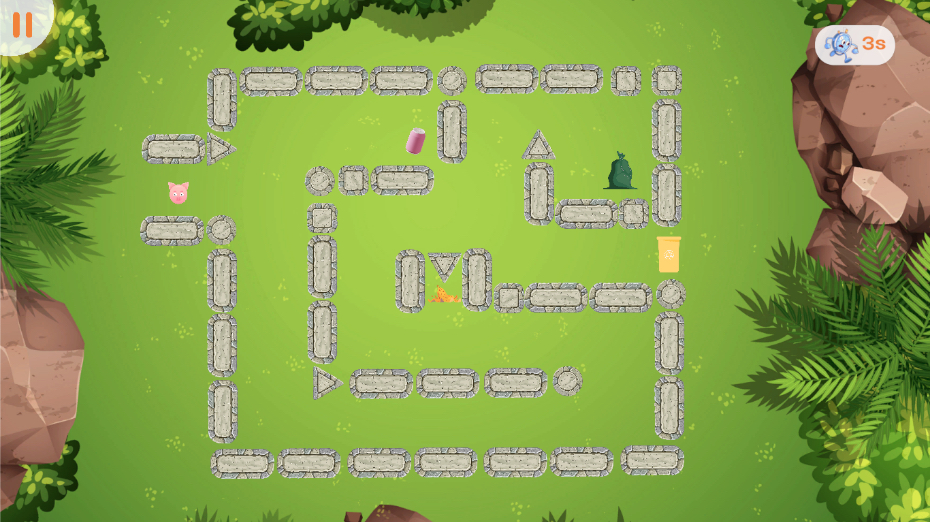
\includegraphics[scale=0.45]{Chapters/gameplay/MazeGame.jpg}
    \caption{Maze Game - Gameplay}
    \label{fig:mazeGameplay}    
\end{figure}

\newpage
\section{Game 3 - Sounds}

The Sounds Game is designed for children aged 4 to 10 years old.

\paragraph{Description}
This game is a playful and interactive way to help children develop key auditory skills. It consists of a nature environment where there are multiple instruments scattered around it. The player is asked to play a sound and spot the instrument being played in the map.

The primary actions are:

\begin{itemize}
    \item \textbf{Listening} to the sound that is played when the play button is pressed.
    \item \textbf{Identify} the instrument that is currently being played.
    \item \textbf{Find and Select} the instrument previously identified. 
\end{itemize}

% TODO: Consider adding a maximum error threshold

The player is successfull when one is able to correctly identify and find the matching instrument for the sound being played. When this happens, the player is met with positive feedback such as celebratory sounds. On the other hand, some players may encounter some difficulties and will be met with a negative feedback from the game, in the form of error sounds.
As the levels progress, they may increase in complexity with more complex sounds and hard to guess instruments, ensuring engagement and new challenges.

\subsection*{Competences}
The Sounds Game helps with the following competences:

\paragraph{Auditory Discrimination}- The game helps children sharpen their ability to distinguish different sounds, allowing them to listen carefully and to identify the instrument being played. It is particularly helpful for children with \textbf{Auditory Processing Disorder}, training them to differentiate between sounds.

\paragraph{Visual-Auditory Integration}- Children must match the sound they hear with the correct representation of instrument in the game. This is helpful for children with \textbf{Dyslexia} and \textbf{Language Processing Disorder} whose ability to integrate sensory information can be a challenge.

The following image (fig. \ref{fig:soundsGameplay}) displays the aspect of the game during one of the gameplays.
\begin{figure}[H]
    \centering
    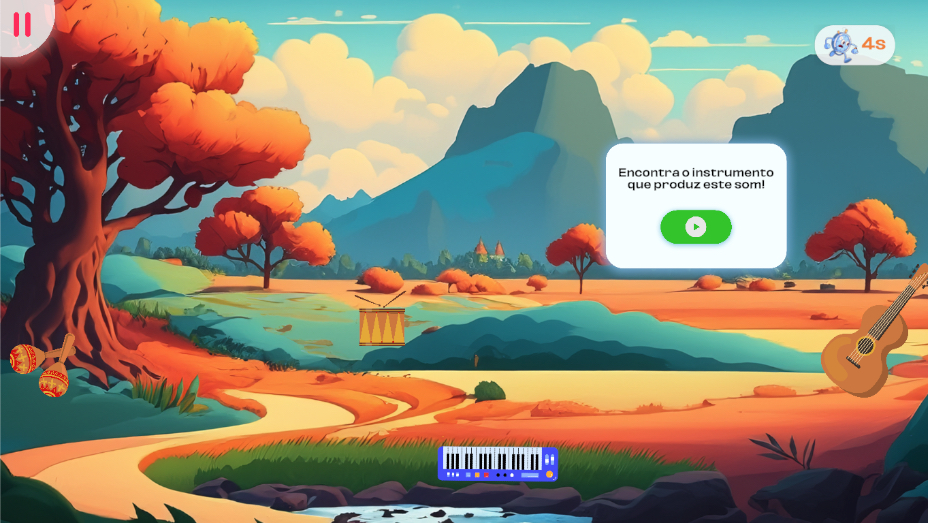
\includegraphics[scale=0.45]{Chapters/gameplay/SoundsGame.jpg}
    \caption{Sounds Game - Gameplay}
    \label{fig:soundsGameplay}    
\end{figure}

\newpage
\section{Game 4 - Words}
The Words Game is designed for children between the age of 6 and 10 years old.

\paragraph{Description}
This game consists of an image and a sequence of characters in which some are blank. The objective is for the player to complete the word with the matching characters.

The primary actions present here are the following:

\begin{itemize}
    \item \textbf{Recognize the image} on the screen.
    \item \textbf{Recognize the word} based on both the image and the displayed letters.
    \item \textbf{Complete the word} by clicking each slot and filling it with each letter.
\end{itemize}

The player is successful by completing the word correctly. When this is accomplished, a success sound plays and shows the score to the player, encouraging the player to move to different levels.
The player fails when is not able to understand which word the image refers to and therefore is not able to complete it.

\subsection*{Competences}
The Words game helps with the following competences:

\paragraph{Spelling and Vocabulary Building}- Completing words based on given images provides the children a chance to expand their vocabulary. This competence is really valuable for children with \textbf{Dysgraphia} and \textbf{Dyslexia}, that can often struggle with new vocabulary and spelling.

\paragraph{Memory}- Playing the game and completing words requires the players to use their memory to recall words, strengthening the ability to remember information. This is particularly valuable for children with \textbf{Dyscalculia}.

The following image (fig. \ref{fig:wordsGameplay}) represents a screenshot of one of the gameplays.

\begin{figure}[H]
    \centering
    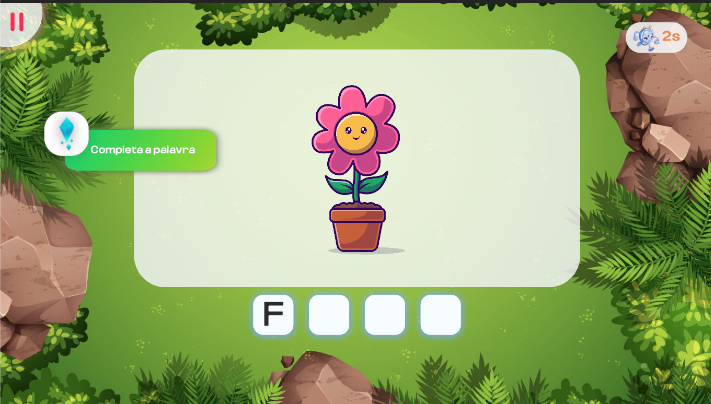
\includegraphics[scale=0.45]{Chapters/gameplay/WordsGame.jpg}
    \caption{Words Game - Gameplay}
    \label{fig:wordsGameplay}    
\end{figure}

\newpage
\section{Game 5 - Puzzle}

The Puzzle Game is designed for children aged from 5 to 12 years old.

\paragraph{Description}

In the Puzzles Game, the user has multiple levels each one with different images related to ecology. The player can choose the difficulty level to play. The difficulty levels are: Easy, Medium, and Hard (3x3, 4x4, 5x5). Inside the game level the player will have a small window with a view of the completed puzzle, as well as a puzzle section composed by the puzzle table and a tray with puzzle pieces.
The objective is for the player to drag the puzzle pieces present on the tray and to drop them in the puzzle table in the correct places. After reaching the end of the puzzle, the game plays a success notification to let the user know it's correct.

The primary actions are:

\begin{itemize}
    \item \textbf{Analyze the image} of the puzzle.
    \item \textbf{Place the pieces} from the tray on the puzzle table.
\end{itemize}

The score is measured like other games, with a timer. There's no time limit so success would be for a child to complete the puzzle as fast as possible. Failure can also happen, although no time limit is applied. This may happen when the player struggles too much with the placement of the pieces in the right place and gives up. In this case, it's suggested that the player should choose an easier level.

\subsection*{Competences}

The Puzzle Game can help with the development of the following competences:

\paragraph{Fine Motor Skills}- Dragging and dropping the pieces into place can require precise control of fine motor skills. This is mostly important for children with \textbf{Dysgraphia} and \textbf{Visual Motor Deficit} who struggle with motor coordination tasks.

\paragraph{Problem Solving and Critical Thinking}- When solving each puzzle, children are encouraged to think critically about the correct placement of each piece. They are forced to analyze and match each piece to its correspondant place. This is beneficial for children with \textbf{Dyslexia} and \textbf{Dyscalculia} that are challenged in cognitive processing.

\paragraph{Patience}- Completing a puzzle can require a lot of patience and the ability to handle small frustrations, when something doesn't go the way we want it to go. This is a valuable competence for all children but particularly for children with \textbf{Non-Verbal Learning Disabilities}.

The image \ref{fig:puzzleGameplay} represents the gameplay of the Puzzle Game.

\begin{figure}[H]
    \centering
    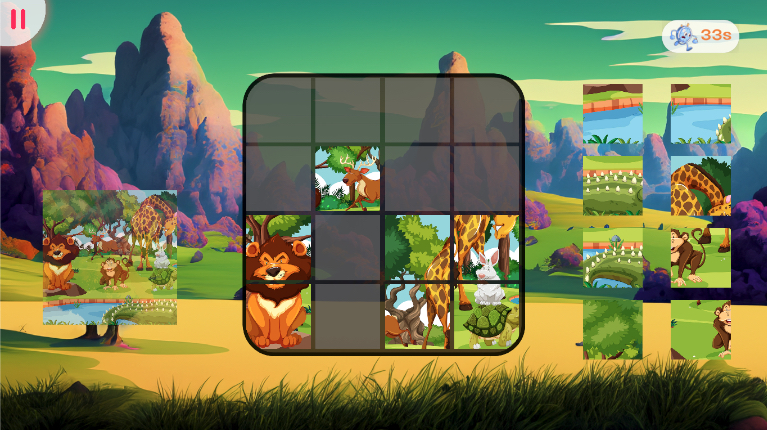
\includegraphics[scale=0.45]{Chapters/gameplay/PuzzleGame.jpg}
    \caption{Puzzle Game - Gameplay}
    \label{fig:puzzleGameplay}    
\end{figure}